\section{Rules that read two neighbours: the classes of 63 and 187}\label{sec:halfradius}

The rules of the classes $\{63,119,238,252\}$ and $\{187,207,221,243\}$ are not permutive in an outer variable, and the front method of Section~\ref{sec:rigidity30} does not apply to them. They have another feature: the local rule ignores one of the two outer neighbours. We show that this alone makes the automorphism group as small as possible.

\begin{theorem}\label{hr:thm:main}
Let $f$ be one of the eight rules
\[
63,\ 119,\ 238,\ 252,\qquad 187,\ 207,\ 221,\ 243,
\]
and $F=F_f$. Then $\Aut(X_F)=\langle\sh\rangle\times\langle F\rangle\cong\Z^2$: every invertible block map commuting with $F$ equals $\sh^aF^b$ for exactly one $(a,b)\in\Z^2$. There is no bound on the radius.
\end{theorem}

The proof has two parts. In the first (Sections~\ref{hr:sec:setting}--\ref{hr:sec:offset}) the rightmost difference between two configurations is shown to be invariant under $F$, every automorphism $h$ is shown to move it by a constant $e(h)$, and $h$ is reduced to $\sh^{e(h)}h$, an automorphism that, like its inverse, reads only cells to its right. The constancy of $e(h)$ comes from a maximum principle and the strong connectivity of a window graph $W_M$, which we prove for every $M$ by identifying the window graphs with the action of a self-similar group on the $4$-ary tree (Section~\ref{hr:sec:tree}). In the second part (Section~\ref{hr:sec:kernel}) the automorphisms $h$ with $e(h)=0$ are shown to be exactly the powers of $F$, by an induction on the anticipation. A consequence is that $F$ defines an automorphism of the one-sided full shift $\A^{\mathbb N}$ whose centralizer in $\Aut(\A^{\mathbb N})$ is generated by it (Corollary~\ref{hr:cor:onesided}). The proof is by hand. It contains three finite checks, each set out in a table: the cell permutations commuting with $F$ (Lemma~\ref{hr:lem:P}), two section identities in the tree group (Lemma~\ref{hr:lem:sections}), and the level-$1$ groups generated by two permutations of four letters (Lemma~\ref{hr:lem:level1}). They are marked \emph{(finite check)} where they occur.

\subsection{The half-radius form}\label{hr:sec:setting}

Throughout this section $\Aut(X_F)$ is identified with the group of invertible block maps commuting with $F$ (Lemma~\ref{lem:spacetime}). Let $\kappa(c)_i=(1\oplus x_i,1\oplus y_i)$ be the cellwise complement and $\mathrm{rev}(c)_i=c_{-i}$ the reflection; both are involutions. By \eqref{eq:F}, $\kappa F_f\kappa=F_{f'}$ with $f'(a,b,c)=f(\neg a,\neg b,\neg c)$, and $\mathrm{rev}\,F_f\,\mathrm{rev}=F_{f'}$ with $f'(a,b,c)=f(c,b,a)$; moreover $\kappa\sh\kappa=\sh$ and $\mathrm{rev}\,\sh\,\mathrm{rev}=\sh^{-1}$. So conjugation by $\kappa$, and by $\mathrm{rev}$, maps $\Aut(X_{F_f})$ onto $\Aut(X_{F_{f'}})$ and $\langle\sh,F_f\rangle$ onto $\langle\sh,F_{f'}\rangle$. Rule $63$ is $\neg(a\wedge b)$, its reflection $119$ is $\neg(b\wedge c)$, and $\kappa$ maps $119$ to $238=b\vee c$, whose reflection is $252=a\vee b$. Rule $187$ is $\neg b\vee c$, its reflection $243$ is $a\vee\neg b$, and $\kappa$ maps $187$ to $221=b\vee\neg c$, whose reflection is $207=\neg a\vee b$. So it suffices to prove Theorem~\ref{hr:thm:main} for $f=119$ and $f=187$. Both have the form
\[
f(a,b,c)=g(b,c),\qquad g(y,\nu)=\begin{cases}\neg(y\wedge \nu)&(f=119),\\ \neg y\vee \nu&(f=187).\end{cases}
\]
For a cell $z=(x,y)$ write $x(z)=x$, $y(z)=y$, and, for $\nu\in\{0,1\}$,
\[
\phi_\nu(x,y)=\bigl(y,\ x\oplus g(y,\nu)\bigr),\qquad \psi_\nu(x,y)=\bigl(y\oplus g(x,\nu),\ x\bigr).
\]
By \eqref{eq:F} and \eqref{eq:Finv},
\begin{equation}\label{hr:eq:half}
F(c)_i=\phi_{y(c_{i+1})}(c_i),\qquad F^{-1}(d)_i=\psi_{x(d_{i+1})}(d_i).
\end{equation}
Each $\phi_\nu$ and each $\psi_\nu$ is a permutation of the four cells. Table~\ref{hr:tab:phi} lists the values of $\phi_0$ and $\phi_1$, with the cells written as $z=2x+y$; all the finite checks of this section are read off from it.

\begin{table}[ht]
\centering
\begin{tabular}{llccccl}
\toprule
$f$ & & $z=0$ & $1$ & $2$ & $3$ & cycles\\
\midrule
$187$ & $\phi_0$\quad($g(y,0)=\neg y$) & $1$ & $2$ & $0$ & $3$ & $(0\,1\,2)$\\
& $\phi_1$\quad($g(y,1)=1$) & $1$ & $3$ & $0$ & $2$ & $(0\,1\,3\,2)$\\
\midrule
$119$ & $\phi_0$\quad($g(y,0)=1$) & $1$ & $3$ & $0$ & $2$ & $(0\,1\,3\,2)$\\
& $\phi_1$\quad($g(y,1)=\neg y$) & $1$ & $2$ & $0$ & $3$ & $(0\,1\,2)$\\
\bottomrule
\end{tabular}
\caption{The permutations $\phi_\nu(x,y)=(y,\,x\oplus g(y,\nu))$ of the cells $z=2x+y$: the entry in column $z$ is $\phi_\nu(z)$.}
\label{hr:tab:phi}
\end{table}

We use the following facts, all immediate from \eqref{hr:eq:half} and the definition of $g$.
\begin{enumerate}
\item[(a)] $F(c)_i$ depends only on $c_i$ and $y(c_{i+1})$, and $F^{-1}(d)_i$ only on $d_i$ and $x(d_{i+1})$.
\item[(b)] $x(F(c)_i)=y(c_i)$ and $y(F^{-1}(d)_i)=x(d_i)$.
\item[(c)] For a cell $z$, the map $\nu\mapsto\phi_\nu(z)$ is injective if and only if $y(z)=1$, and $\nu\mapsto\psi_\nu(z)$ is injective if and only if $x(z)=1$. (In both rules $g(0,\cdot)\equiv1$ and $g(1,\cdot)$ is a bijection of $\{0,1\}$.)
\end{enumerate}

\begin{lemma}[finite check]\label{hr:lem:P}
For $f\in\{119,187\}$ the only permutation $\pi$ of $\A$ such that the cellwise map $c\mapsto(\pi(c_i))_i$ commutes with $F$ is the identity.
\end{lemma}

\begin{proof}
On a constant configuration $z^{\Z}$, $F$ acts as the permutation $C(z)=\phi_{y(z)}(z)$ of $\A$. By Table~\ref{hr:tab:phi}, $C=(0\,1\,3\,2)$ for $187$ and $C=(0\,1\,2)$ for $119$. A cellwise $\pi$ commuting with $F$ maps constant configurations to constant configurations, so $\pi C=C\pi$. In $\Sym(\A)$ the $4$-cycles form a conjugacy class of $6$ elements and the $3$-cycles one of $8$ elements, so the centralizer of $C$ has order $24/6=4$ for $187$ and $24/8=3$ for $119$; in both cases it is $\langle C\rangle$. It remains to see that $\pi=C^j\ne\mathrm{id}$ does not commute with $F$. By \eqref{hr:eq:half}, if $\pi$ commutes with $F$, then
\[
\pi\bigl(\phi_{y(c_1)}(c_0)\bigr)=\phi_{y(\pi c_1)}(\pi c_0)\qquad\text{for all cells }c_0,c_1.
\]
Table~\ref{hr:tab:P} gives, for each $\pi=C^j\ne\mathrm{id}$, cells $c_0,c_1$ for which the two sides differ; each evaluation is read off from Table~\ref{hr:tab:phi}.
\end{proof}

\begin{table}[ht]
\centering
\begin{tabular}{llcll}
\toprule
$f$ & $\pi$ & $(c_0,c_1)$ & $\pi(\phi_{y(c_1)}(c_0))$ & $\phi_{y(\pi c_1)}(\pi c_0)$\\
\midrule
$187$ & $C=(0\,1\,3\,2)$ & $(1,0)$ & $\pi(\phi_0(1))=\pi(2)=0$ & $\phi_{y(1)}(3)=\phi_1(3)=2$\\
& $C^2=(0\,3)(1\,2)$ & $(0,1)$ & $\pi(\phi_1(0))=\pi(1)=2$ & $\phi_{y(2)}(3)=\phi_0(3)=3$\\
& $C^3=(0\,2\,3\,1)$ & $(1,0)$ & $\pi(\phi_0(1))=\pi(2)=3$ & $\phi_{y(2)}(0)=\phi_0(0)=1$\\
\midrule
$119$ & $C=(0\,1\,2)$ & $(1,0)$ & $\pi(\phi_0(1))=\pi(3)=3$ & $\phi_{y(1)}(2)=\phi_1(2)=0$\\
& $C^2=(0\,2\,1)$ & $(1,0)$ & $\pi(\phi_0(1))=\pi(3)=3$ & $\phi_{y(2)}(0)=\phi_0(0)=1$\\
\bottomrule
\end{tabular}
\caption{Proof of Lemma~\ref{hr:lem:P}: for each nontrivial power $\pi$ of $C$, a pair of cells $(c_0,c_1)$ at which $\pi\circ F\ne F\circ\pi$.}
\label{hr:tab:P}
\end{table}

\paragraph{The exact right edge.} A \emph{pair} is an ordered pair $Q=(c,c')$ of distinct configurations that agree at all sufficiently large sites, and its \emph{right edge} is $\lambda(Q)=\max\{i:c_i\ne c'_i\}$. As in Section~\ref{sec:rigidity30}, $hQ=(hc,hc')$, $FQ$ and $\sh^jQ$ are pairs whenever $h$ is an invertible block map.

\begin{lemma}\label{hr:lem:edge}
$\lambda(FQ)=\lambda(F^{-1}Q)=\lambda(Q)$ for every pair $Q$, and $\lambda(\sh^jQ)=\lambda(Q)-j$.
\end{lemma}

\begin{proof}
Let $p=\lambda(Q)$. For $i>p$, $F(c)_i$ and $F(c')_i$ depend only on cells at sites $\ge i>p$, where $c=c'$. At $p$, $F(c)_p=\phi_\nu(c_p)$ and $F(c')_p=\phi_\nu(c'_p)$ with the same $\nu=y(c_{p+1})=y(c'_{p+1})$, and $\phi_\nu$ is injective, so they differ. The same argument with $\psi$ applies to $F^{-1}$. The last statement is clear.
\end{proof}

So the right edge of a difference is stationary, in both time directions and in every context. This replaces the light-speed front of the permutive rules.

\subsection{The offset}\label{hr:sec:offset}

In this subsection $h\in\Aut(X_F)$ and $R\ge1$ bounds the radii of $h$ and $h^{-1}$. For a pair $Q$ with $\lambda(Q)=p$ put $E(Q)=\lambda(hQ)-p$.

\begin{lemma}\label{hr:lem:E}
Let $Q=(c,c')$ be a pair with $\lambda(Q)=p$.
\begin{enumerate}
\item $E(Q)\in[-R,R]$, and $E(Q)$ depends only on the restrictions of $c$ and $c'$ to $[p-2R,p+2R]$.
\item $E(\sh^jQ)=E(Q)$, $E(FQ)=E(Q)$ and $E(c',c)=E(c,c')$.
\end{enumerate}
\end{lemma}

\begin{proof}
(1) $hc$ and $hc'$ agree at every site $i>p+R$. If they agreed at every site $i\ge p-R$, then $c_p=h^{-1}(hc)_p=h^{-1}(hc')_p=c'_p$, since $h^{-1}$ has radius at most $R$. So $\lambda(hQ)\in[p-R,p+R]$, and it is the largest site in this interval at which $hc$ and $hc'$ differ. These cells depend only on $c$ and $c'$ on $[p-2R,p+2R]$. (2) By Lemma~\ref{hr:lem:edge} and $hF=Fh$, $\lambda(hFQ)=\lambda(FhQ)=\lambda(hQ)$ and $\lambda(FQ)=\lambda(Q)$; the shift is similar, and $\lambda$ is symmetric in the two configurations.
\end{proof}

Let $e_{\max}$ be the largest value of $E$ over all pairs.

\begin{lemma}[maximum principle]\label{hr:lem:max}
Let $Q=(c,c')$ be a pair with $\lambda(Q)=p$ and $E(Q)=e_{\max}$. If $c''$ agrees with $c'$ at every site $i\ge p$, then $(c,c'')$ is a pair with $\lambda(c,c'')=p$ and $E(c,c'')=e_{\max}$. The same holds with the roles of $c$ and $c'$ exchanged.
\end{lemma}

\begin{proof}
Clearly $\lambda(c,c'')=p$. Let $c^*$ agree with $c''$ on $[p-2R,\infty)$ and with $c'$ elsewhere. By Lemma~\ref{hr:lem:E}(1), $E(c,c^*)=E(c,c'')$. The configurations $c'$ and $c^*$ differ at finitely many sites, all in $[p-2R,p-1]$. Change them one site at a time, $c'=c^0,c^1,\dots,c^n=c^*$, so that $Q_k=(c^{k-1},c^k)$ is a pair with $\lambda(Q_k)=\ell_k\le p-1$. Then $\lambda(hQ_k)=\ell_k+E(Q_k)\le p-1+e_{\max}$, so $hc^{k-1}$ and $hc^k$ agree at all sites $\ge p+e_{\max}$, for every $k$. Hence $hc^*$ agrees with $hc'$ at all sites $\ge p+e_{\max}$. Since $hc$ and $hc'$ differ at $p+e_{\max}$ and agree beyond it, so do $hc$ and $hc^*$, that is, $E(c,c^*)=e_{\max}$. The last statement follows from $E(c',c)=E(c,c')$.
\end{proof}

Unlike Lemma~\ref{r30:lem:max}, this is instantaneous: no time evolution is needed, because the right edge of a difference does not move.

\begin{corollary}\label{hr:cor:word}
Let $M=2R$. Whether $E(Q)=e_{\max}$ for a pair $Q=(c,c')$ with $\lambda(Q)=p$ depends only on the word $c_p\cdots c_{p+M}$ and the cell $c'_p$.
\end{corollary}

\begin{proof}
By Lemma~\ref{hr:lem:E}(2) we may compare pairs $Q_1=(c_1,c'_1)$ and $Q_2=(c_2,c'_2)$ with the same right edge $p$, with $c_1=c_2$ on $[p,p+M]$ and $(c'_1)_p=(c'_2)_p$, and suppose $E(Q_1)=e_{\max}$. Let $c_3$, $c'_3$ agree with $c_1$, $c'_1$ on $(-\infty,p+M]$ and with $c_2$ beyond. Then $Q_3=(c_3,c'_3)$ is a pair with right edge $p$ that agrees with $Q_1$ on $[p-2R,p+2R]$, so $E(Q_3)=e_{\max}$. Since $c_3=c_2$ on $[p,\infty)$, Lemma~\ref{hr:lem:max} with the roles exchanged gives $E(c_2,c'_3)=e_{\max}$. Since $c'_3=c_2'$ on $[p,\infty)$, Lemma~\ref{hr:lem:max} gives $E(c_2,c'_2)=e_{\max}$.
\end{proof}

\begin{definition}\label{hr:def:graphs}
Fix $M\ge0$. For $\nu\in\{0,1\}$ and a word $\omega=\omega_0\cdots\omega_M\in\A^{M+1}$ let $F_\nu(\omega)$ be the word of $F(\tilde c)$ on $[p,p+M]$, where $\tilde c$ has the word $\omega$ on $[p,p+M]$ and $y(\tilde c_{p+M+1})=\nu$; by \eqref{hr:eq:half}, $F_\nu(\omega)_k=\phi_{y(\omega_{k+1})}(\omega_k)$ for $k<M$ and $F_\nu(\omega)_M=\phi_\nu(\omega_M)$. The \emph{window graph} $\Lambda^0_M$ (the front does not move; this is not the light-speed graph $\Lambda_M$ of Section~\ref{r30:sec:window}) has vertex set $\A^{M+1}$ and the edges $\omega\to F_\nu(\omega)$, $\nu\in\{0,1\}$. The \emph{two-copy window graph} $W_M$ has as vertices the pairs $(\omega,z)$ with $\omega\in\A^{M+1}$, $z\in\A$, $z\ne\omega_0$, and the edges
\[
(\omega,z)\longrightarrow\bigl(F_\nu(\omega),\ \phi_{y(\omega_1)}(z)\bigr),\qquad \nu\in\{0,1\},
\]
with $\phi_{y(\omega_1)}$ replaced by $\phi_\nu$ if $M=0$.
\end{definition}

A vertex $(\omega,z)$ of $W_M$ records a pair $(c,c')$ with right edge $p$: the word of $c$ on $[p,p+M]$, which is also that of $c'$ on $[p+1,p+M]$, and the cell $c'_p=z$. An edge applies $F$ to both, with the input $\nu$ entering from the right; the new second cell is $F(c')_p=\phi_{y(c_{p+1})}(z)$, which differs from $F(c)_p$.

\begin{proposition}\label{hr:prop:offset}
Suppose that $W_{2R}$ is strongly connected. Then $E$ is constant: there is $e(h)\in[-R,R]$ with $\lambda(hQ)=\lambda(Q)+e(h)$ for every pair $Q$.
\end{proposition}

\begin{proof}
Let $M=2R$ and let $\mathcal S$ be the set of vertices $(\omega,z)$ of $W_M$ such that $E(Q)=e_{\max}$ for some, equivalently (Corollary~\ref{hr:cor:word}) every, pair $Q=(c,c')$ with right edge $p$, word $\omega$ of $c$ on $[p,p+M]$ and $c'_p=z$. Every vertex is realised by some pair, so $\mathcal S\ne\emptyset$. If $(\omega,z)\in\mathcal S$ and $\nu\in\{0,1\}$, choose such a pair with $y(c_{p+M+1})=\nu$. Then $FQ$ has right edge $p$ (Lemma~\ref{hr:lem:edge}), $E(FQ)=E(Q)=e_{\max}$, and $FQ$ realises the successor of $(\omega,z)$ along the edge labelled $\nu$. So $\mathcal S$ is forward-closed, and by strong connectivity it is everything. Put $e(h)=e_{\max}$.
\end{proof}

\begin{corollary}\label{hr:cor:reduce}
Suppose that $W_M$ is strongly connected for every $M$. Then:
\begin{enumerate}
\item $e\colon\Aut(X_F)\to\Z$ is a homomorphism, with $e(\sh)=-1$ and $e(F)=0$, and $e(h)$ does not depend on $R$;
\item if $e(h)=0$, then there are $A\ge0$ and $K\colon\A^{A+1}\to\A$ with $h(c)_i=K(c_i,\dots,c_{i+A})$ for all $c$ and $i$, and $K$ is a bijection in its first argument when the others are fixed; the same holds for $h^{-1}$;
\item $\Aut(X_F)=\langle\sh\rangle\times\ker e$, the isomorphism being $h\mapsto(\sh^{-e(h)},\,\sh^{e(h)}h)$.
\end{enumerate}
\end{corollary}

\begin{proof}
(1) $\lambda(h_1h_2Q)=\lambda(h_2Q)+e(h_1)=\lambda(Q)+e(h_2)+e(h_1)$; the values on $\sh$ and $F$ are Lemma~\ref{hr:lem:edge}. (2) Let $e(h)=0$ and let $R$ bound the radii of $h$ and $h^{-1}$. If $c$ and $c'$ differ only at sites $<i$, then $\lambda(hc,hc')=\lambda(c,c')<i$, so $h(c)_i=h(c')_i$: the cell $h(c)_i$ does not depend on the cells left of $i$, and so $h(c)_i=K(c_{[i,i+A]})$ with $A\le R$. If $c$ and $c'$ differ only at $i$, then $\lambda(hc,hc')=i$, so $h(c)_i\ne h(c')_i$; hence $K$ is injective, so bijective, in its first argument. Since $e(h^{-1})=-e(h)=0$, the same holds for $h^{-1}$. (3) $\sh$ commutes with every block map, $e(\sh^ah)=e(h)-a$, and $\langle\sh\rangle\cap\ker e=\{\mathrm{id}\}$.
\end{proof}

For $h\in\ker e$ the least $A$ in (2) is the \emph{anticipation} $A(h)$. If $A(h)=0$, then $h$ is a cellwise permutation commuting with $F$, so $h=\mathrm{id}$ by Lemma~\ref{hr:lem:P}.

\subsection{The window graphs as a self-similar group}\label{hr:sec:tree}

We write words of $\Lambda^0_M$ backwards: the word $\omega_0\cdots\omega_M$ on $[p,p+M]$ is the vertex $\bar\omega=\omega_M\omega_{M-1}\cdots\omega_0$ of level $M+1$ of the rooted $4$-ary tree $\A^*$, so that the first letter is the cell next to the incoming bit. Let $s_0$ and $s_1$ be the maps of $\A^*$ to itself given by
\[
s_\nu(xw)=\phi_\nu(x)\,s_{y(x)}(w)\qquad(x\in\A,\ w\in\A^*),
\]
so that $s_\nu(\bar\omega)=\overline{F_\nu(\omega)}$ by Definition~\ref{hr:def:graphs}. These are the maps computed by the two states of the Mealy automaton of Figure~\ref{hr:fig:mealy}: in the state $s_\nu$ the automaton reads a letter $x$, writes $\phi_\nu(x)$ and passes to the state $s_{y(x)}$. Each $s_\nu$ is a bijection on every level, and we put $G=\langle s_0,s_1\rangle$. We use the standard language of self-similar groups \cite{Nekrashevych2005}. For $t\in G$ and a letter $x$ there are $t(x)\in\A$ and $t|_x\in G$, the \emph{section} of $t$ at $x$, with $t(xw)=t(x)\,t|_x(w)$ for all $w\in\A^*$; for a word $u=x_1\cdots x_m$ the section at $u$ is $t|_u=(\cdots(t|_{x_1})|_{x_2}\cdots)|_{x_m}$, so that $t(uw)=t(u)\,t|_u(w)$. The sections of the generators do not depend on the generator: $s_\nu|_x=s_{y(x)}$. Sections satisfy the product rule $(tt')|_x=t|_{t'(x)}\,t'|_x$ and $t^{-1}|_x=(t|_{t^{-1}(x)})^{-1}$. The \emph{level-$1$ image} of a subgroup of $G$ is its image in $\Sym(\A)$ under $t\mapsto(x\mapsto t(x))$; that of $s_\nu$ is $\phi_\nu$.

\begin{figure}[ht]
\centering
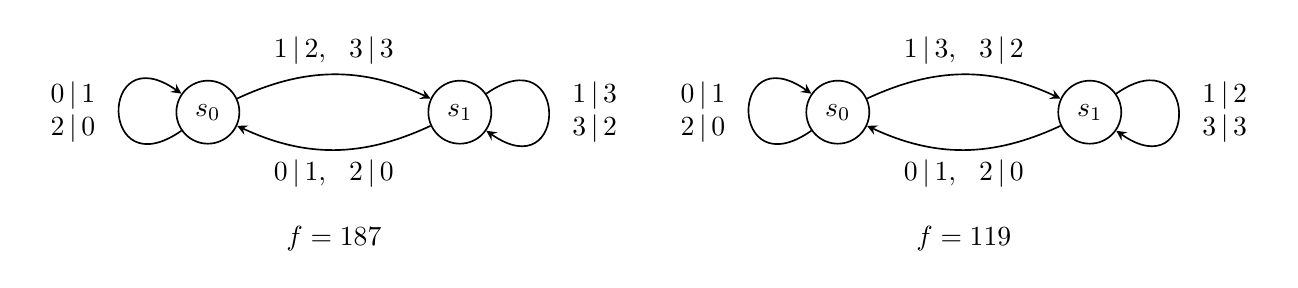
\begin{tikzpicture}[>=stealth,semithick,state/.style={circle,draw,minimum size=8mm,inner sep=0pt}]
\begin{scope}
\node[state] (a0) at (0,0) {$s_0$};
\node[state] (a1) at (3.2,0) {$s_1$};
\draw[->] (a0) to[out=215,in=145,looseness=7] node[left] {$\begin{array}{c}0\,|\,1\\2\,|\,0\end{array}$} (a0);
\draw[->] (a1) to[out=35,in=-35,looseness=7] node[right] {$\begin{array}{c}1\,|\,3\\3\,|\,2\end{array}$} (a1);
\draw[->] (a0) to[bend left=25] node[above] {$1\,|\,2,\ \ 3\,|\,3$} (a1);
\draw[->] (a1) to[bend left=25] node[below] {$0\,|\,1,\ \ 2\,|\,0$} (a0);
\node at (1.6,-1.6) {$f=187$};
\end{scope}
\begin{scope}[xshift=8cm]
\node[state] (b0) at (0,0) {$s_0$};
\node[state] (b1) at (3.2,0) {$s_1$};
\draw[->] (b0) to[out=215,in=145,looseness=7] node[left] {$\begin{array}{c}0\,|\,1\\2\,|\,0\end{array}$} (b0);
\draw[->] (b1) to[out=35,in=-35,looseness=7] node[right] {$\begin{array}{c}1\,|\,2\\3\,|\,3\end{array}$} (b1);
\draw[->] (b0) to[bend left=25] node[above] {$1\,|\,3,\ \ 3\,|\,2$} (b1);
\draw[->] (b1) to[bend left=25] node[below] {$0\,|\,1,\ \ 2\,|\,0$} (b0);
\node at (1.6,-1.6) {$f=119$};
\end{scope}
\end{tikzpicture}
\caption{The Mealy automata defining $s_0$ and $s_1$. An arrow from $s_\nu$ labelled $x\,|\,z$ means that in the state $s_\nu$ the letter $x$ is replaced by $z=\phi_\nu(x)$ (Table~\ref{hr:tab:phi}); the arrow ends at $s_{y(x)}$, the state in which the next letter is read. The letters are the cells $2x+y$, so the arrows into $s_0$ carry the inputs $0,2$ and those into $s_1$ the inputs $1,3$.}
\label{hr:fig:mealy}
\end{figure}

Since the edges of $\Lambda^0_M$ are the two permutations $s_0,s_1$ of the finite level $M+1$, and the inverse of a permutation of a finite set is a positive power of it, $\Lambda^0_M$ is strongly connected if and only if $G$ acts transitively on level $M+1$. Likewise, by Definition~\ref{hr:def:graphs}, a vertex $(\omega,z)$ of $W_M$ is the ordered pair of distinct \emph{siblings} $\bar\omega=u\,\omega_0$ and $u\,z$ of level $M+1$, with common parent $u=\omega_M\cdots\omega_1$ of level $M$, and an edge applies the same generator to both. Hence:

\begin{lemma}\label{hr:lem:Wtree}
$W_M$ is strongly connected if and only if $G$ acts transitively on ordered pairs of distinct siblings of level $M+1$. This holds if $G$ is transitive on level $M$ and, for one vertex $u$ of level $M$, the level-$1$ image of $\{t|_u:t\in G,\ t(u)=u\}$ is $2$-transitive on $\A$.
\end{lemma}

\begin{proof}
The first statement is the remark above. For the second, given ordered sibling pairs $(vx,vz)$ and $(v'x',v'z')$, move $v$ and $v'$ to $u$ by elements of $G$, and then $(x,z)$ to $(x',z')$ by an element of the stabilizer of $u$, which acts on the children of $u$ through its sections at $u$.
\end{proof}

Let $H=\langle s_0^2,s_1\rangle\le G$, and let $x_*=1$ for $f=187$ and $x_*=3$ for $f=119$. Words in $s_0^{\pm1},s_1^{\pm1}$ are composed from right to left.

\begin{lemma}[finite check: section identities]\label{hr:lem:sections}
The following elements of $H$ fix the letter $x_*$ and have the stated sections at $x_*$:
\begin{center}
\begin{tabular}{lll}
\toprule
$f$ & element & section at $x_*$\\
\midrule
$187$, $x_*=1$ & $t_1=s_1s_0^{-2}s_1^2$ & $s_1$\\
& $t_2=s_0^2s_1s_0^{-2}s_1$ & $s_0^2$\\
\midrule
$119$, $x_*=3$ & $t_1=s_1$ & $s_1$\\
& $t_2=s_0^{-2}s_1^3s_0^2$ & $s_0^2s_1$\\
\bottomrule
\end{tabular}
\end{center}
\end{lemma}

\begin{proof}
All four elements are words in $s_0^{\pm2}$ and $s_1^{\pm1}$, so they lie in $H$. By the rules for sections, $s_\nu|_x=s_{y(x)}$, and $s_\nu^{-1}|_x=(s_{y(x')})^{-1}$ with $x'=\phi_\nu^{-1}(x)$. For $f=119$ and $t_1=s_1$: $\phi_1(3)=3$ and $s_1|_3=s_{y(3)}=s_1$. For the other three elements, Table~\ref{hr:tab:sections} follows the letter $x_*$ through the word, from the rightmost generator to the leftmost. Each row gives the generator applied, the letter before and after it (read off from Table~\ref{hr:tab:phi}), and the section of that generator at the letter before it. In each case the last letter is $x_*$. By the product rule, the section of the word at $x_*$ is the product of the sections in the table, taken from the last row on the left to the first row on the right; the last line of each block gives this product and its reduction.
\end{proof}

\begin{table}[ht]
\centering
\small
\begin{tabular}{lcl}
\toprule
\multicolumn{3}{l}{$187$:\quad $t_1=s_1s_0^{-2}s_1^2$}\\
\midrule
step & letter & section\\
\midrule
$s_1$ & $1\mapsto3$ & $s_1$\\
$s_1$ & $3\mapsto2$ & $s_1$\\
$s_0^{-1}$ & $2\mapsto1$ & $s_1^{-1}$\\
$s_0^{-1}$ & $1\mapsto0$ & $s_0^{-1}$\\
$s_1$ & $0\mapsto1$ & $s_0$\\
& & \\
& & \\
\midrule
\multicolumn{3}{l}{$s_0\,s_0^{-1}\,s_1^{-1}\,s_1\,s_1=s_1$}\\
\bottomrule
\end{tabular}
\quad
\begin{tabular}{lcl}
\toprule
\multicolumn{3}{l}{$187$:\quad $t_2=s_0^2s_1s_0^{-2}s_1$}\\
\midrule
step & letter & section\\
\midrule
$s_1$ & $1\mapsto3$ & $s_1$\\
$s_0^{-1}$ & $3\mapsto3$ & $s_1^{-1}$\\
$s_0^{-1}$ & $3\mapsto3$ & $s_1^{-1}$\\
$s_1$ & $3\mapsto2$ & $s_1$\\
$s_0$ & $2\mapsto0$ & $s_0$\\
$s_0$ & $0\mapsto1$ & $s_0$\\
& & \\
\midrule
\multicolumn{3}{l}{$s_0\,s_0\,s_1\,s_1^{-1}\,s_1^{-1}\,s_1=s_0^2$}\\
\bottomrule
\end{tabular}
\quad
\begin{tabular}{lcl}
\toprule
\multicolumn{3}{l}{$119$:\quad $t_2=s_0^{-2}s_1^3s_0^2$}\\
\midrule
step & letter & section\\
\midrule
$s_0$ & $3\mapsto2$ & $s_1$\\
$s_0$ & $2\mapsto0$ & $s_0$\\
$s_1$ & $0\mapsto1$ & $s_0$\\
$s_1$ & $1\mapsto2$ & $s_1$\\
$s_1$ & $2\mapsto0$ & $s_0$\\
$s_0^{-1}$ & $0\mapsto2$ & $s_0^{-1}$\\
$s_0^{-1}$ & $2\mapsto3$ & $s_1^{-1}$\\
\midrule
\multicolumn{3}{l}{$s_1^{-1}s_0^{-1}\,s_0\,s_1\,s_0\,s_0\,s_1=s_0^2s_1$}\\
\bottomrule
\end{tabular}
\caption{Proof of Lemma~\ref{hr:lem:sections}. The generators of each word are applied from right to left, starting at the letter $x_*$ ($x_*=1$ for $187$, $x_*=3$ for $119$). A step $s_\nu$ maps the letter $x$ to $\phi_\nu(x)$ with section $s_{y(x)}$; a step $s_\nu^{-1}$ maps $x$ to $x'=\phi_\nu^{-1}(x)$ with section $s_{y(x')}^{-1}$.}
\label{hr:tab:sections}
\end{table}

\begin{lemma}[finite check: level-$1$ groups]\label{hr:lem:level1}
The level-$1$ image of $H$ is $\langle\phi_0^2,\phi_1\rangle$, which is $\Sym(\A)\cong S_4$ for $187$ and the alternating group $A_4$ for $119$. Both are transitive and $2$-transitive on $\A$.
\end{lemma}

\begin{proof}
The level-$1$ images of $s_0^2$ and $s_1$ are $\phi_0^2$ and $\phi_1$; they are listed in Table~\ref{hr:tab:level1}. For $187$, $\phi_0^2$ is a $3$-cycle and $\phi_1$ a $4$-cycle, so the order of the group they generate is divisible by $12$, and the group contains an odd permutation; so it is $S_4$. For $119$, $\phi_0^2$ and $\phi_1$ are even. Conjugating $\phi_0^2=(0\,3)(1\,2)$ by $\phi_1$ gives $(1\,3)(0\,2)$, and the product of the two is $(0\,1)(2\,3)$, so the group contains the Klein four-group and a $3$-cycle; its order is divisible by $12$, and it is $A_4$. Both $S_4$ and $A_4$ are $2$-transitive on four points: they are transitive, and the stabilizer of a point contains a $3$-cycle, which permutes the other three points cyclically.
\end{proof}

\begin{table}[ht]
\centering
\begin{tabular}{llllll}
\toprule
$f$ & $\phi_0^2$ & $\phi_1$ & orders & signs & $\langle\phi_0^2,\phi_1\rangle$\\
\midrule
$187$ & $(0\,2\,1)$ & $(0\,1\,3\,2)$ & $3$, $4$ & even, odd & $S_4$\\
$119$ & $(0\,3)(1\,2)$ & $(0\,1\,2)$ & $2$, $3$ & even, even & $A_4$\\
\bottomrule
\end{tabular}
\caption{Proof of Lemma~\ref{hr:lem:level1}: the level-$1$ images of the generators $s_0^2$, $s_1$ of $H$, from Table~\ref{hr:tab:phi}.}
\label{hr:tab:level1}
\end{table}

\begin{proposition}\label{hr:prop:tree}
For $f\in\{119,187\}$:
\begin{enumerate}
\item $H$ is self-replicating at $x_*$: for every $t\in H$ there is $t'\in H$ with $t'(x_*)=x_*$ and $t'|_{x_*}=t$; consequently, for every $m\ge0$ and $t\in H$ there is $t'\in H$ with $t'(x_*^m)=x_*^m$ and $t'|_{x_*^m}=t$;
\item $H$, and hence $G$, acts transitively on every level, so $\Lambda^0_M$ is strongly connected for every $M$;
\item $W_M$ is strongly connected for every $M\ge0$.
\end{enumerate}
\end{proposition}

\begin{proof}
(1) On the stabilizer of $x_*$ in $H$, the map $t\mapsto t|_{x_*}$ is a homomorphism, by the product rule for sections. By Lemma~\ref{hr:lem:sections} its image contains $s_1$ and $s_0^2$ (for $119$, $s_0^2=(s_0^2s_1)s_1^{-1}$), hence all of $H$. For $m\ge1$ argue by induction: given $t$, choose $t'\in H$ fixing $x_*$ with $t'|_{x_*}=t$, and $t''\in H$ fixing $x_*^{m}$ with $t''|_{x_*^m}=t'$; then $t''$ fixes $x_*^{m+1}$ and $t''|_{x_*^{m+1}}=t'|_{x_*}=t$. (2) By induction on the level $n$. For $n=1$ this is Lemma~\ref{hr:lem:level1}. Given words $xv$ and $x'v'$ of level $n+1$, choose $t\in H$ with $t(x)=x_*$ and $t'\in H$ with $t'(x')=x_*$, so that the words become $x_*w$ and $x_*w'$; by (1) and the induction hypothesis some element of $H$ fixing $x_*$ has a section mapping $w$ to $w'$. (3) By (2), $G$ is transitive on level $M$. By (1), the sections at $u=x_*^M$ of the elements of $H$ fixing $u$ form all of $H$, whose level-$1$ image is $2$-transitive by Lemma~\ref{hr:lem:level1}. Lemma~\ref{hr:lem:Wtree} applies.
\end{proof}

In the terminology of \cite{Nekrashevych2005}, (1) and (2) say that $H$ is self-replicating and level-transitive. For $119$ the level-$1$ image of $G$ is $S_4$, since $\phi_0$ is a $4$-cycle, while that of $H$ is $A_4$; by Lemma~\ref{hr:lem:level1} the smaller group suffices.

\subsection{The kernel of the offset}\label{hr:sec:kernel}

By Proposition~\ref{hr:prop:tree}(3) and Corollary~\ref{hr:cor:reduce}, $\Aut(X_F)=\langle\sh\rangle\times\ker e$, and every $h\in\ker e$ reads only cells to its right: $h(c)_i=K(c_{[i,i+A]})$ with $A=A(h)$ and $K$ bijective in its first argument. We show $\ker e=\langle F\rangle$. Throughout, $h$, $h_1$, $h_2$ denote elements of $\ker e$ with local rules $K$, $K_1$, $K_2$, and $F^{\pm1}\in\ker e$ by Corollary~\ref{hr:cor:reduce}(1).

\paragraph{Tops.} Let $A=A(h)\ge1$. For $\epsilon=(\epsilon_0,\dots,\epsilon_{A-1})\in\A^A$ let $\vartheta_\epsilon\colon\A\to\A$, $\vartheta_\epsilon(z)=K(\epsilon_0,\dots,\epsilon_{A-1},z)$, be the dependence of $K$ on its last argument when the first $A$ arguments are $\epsilon$. Since $A$ is minimal, some $\vartheta_\epsilon$ is not constant.

\begin{lemma}[diagonal top]\label{hr:lem:top}
Let $A(h)\ge1$. For every $\epsilon\in\A^A$ there are maps $\alpha_\epsilon,\beta_\epsilon\colon\{0,1\}\to\{0,1\}$ with $\vartheta_\epsilon(z)=\bigl(\alpha_\epsilon(x(z)),\,\beta_\epsilon(y(z))\bigr)$.
\end{lemma}

\begin{proof}
Let $c$ have $c_{[1,A]}=\epsilon$, that is $c_{1+j}=\epsilon_j$, and $c_{A+1}=z$; the cell $c_0$ is chosen below. By \eqref{hr:eq:half},
\[
(Fh)(c)_0=\phi_{y(h(c)_1)}\bigl(h(c)_0\bigr)=\phi_{y(\vartheta_\epsilon(z))}\bigl(K(c_0,\epsilon)\bigr).
\]
On the other side, $(hF)(c)_0=K(F(c)_{[0,A]})$, and by (a) the cells $F(c)_j$ with $j<A$ do not involve $z$, while $F(c)_A=\phi_{y(z)}(c_A)$ involves $z$ only through $y(z)$. Since $K$ is bijective in its first argument, we may choose $c_0$ with $y(K(c_0,\epsilon))=1$. Then $\nu\mapsto\phi_\nu(K(c_0,\epsilon))$ is injective by (c), and $hF=Fh$ shows that $y(\vartheta_\epsilon(z))$ is a function of $y(z)$. For the $x$-bit use $hF^{-1}=F^{-1}h$: $(F^{-1}h)(c)_0=\psi_{x(\vartheta_\epsilon(z))}(K(c_0,\epsilon))$, while $(hF^{-1})(c)_0$ involves $z$ only through $x(z)$ by (a); choosing $c_0$ with $x(K(c_0,\epsilon))=1$ and using (c) shows that $x(\vartheta_\epsilon(z))$ is a function of $x(z)$.
\end{proof}

Put $\mathcal X_h=\{\epsilon:\alpha_\epsilon\text{ is not constant}\}$ and $\mathcal Y_h=\{\epsilon:\beta_\epsilon\text{ is not constant}\}$. By minimality of $A$, $\mathcal X_h\cup\mathcal Y_h\ne\emptyset$. Call $h$ of \emph{$y$-type} if $\mathcal Y_h\ne\emptyset=\mathcal X_h$, of \emph{$x$-type} if $\mathcal X_h\ne\emptyset=\mathcal Y_h$, and of \emph{both types} if both are nonempty. A nonconstant map $\{0,1\}\to\{0,1\}$ is a bijection. By \eqref{hr:eq:half}, $F$ has anticipation $1$ and $\vartheta_\epsilon(z)=\phi_{y(z)}(\epsilon_0)$, whose $x$-bit $y(\epsilon_0)$ is constant; so $F$ is of $y$-type, with $\mathcal Y_F=\{\epsilon_0:y(\epsilon_0)=1\}$ by (c). Likewise $F^{-1}$ is of $x$-type with anticipation $1$.

\begin{lemma}\label{hr:lem:FF}
\begin{enumerate}
\item If $h$ is of $x$-type, then $A(hF)\le A(h)$, and if equality holds, $hF$ is of $y$-type.
\item If $h$ is of $y$-type, then $A(hF^{-1})\le A(h)$, and if equality holds, $hF^{-1}$ is of $x$-type.
\end{enumerate}
\end{lemma}

\begin{proof}
(1) Let $A=A(h)$. $(hF)(c)_0=K(F(c)_{[0,A]})$, and since $h$ is of $x$-type, $K$ reads its last argument $F(c)_A$ only through $x(F(c)_A)=y(c_A)$, by (b). The cells $F(c)_j$, $j<A$, read $c_{[0,A]}$, and $c_A$ only through $y(c_A)$ (in $F(c)_{A-1}=\phi_{y(c_A)}(c_{A-1})$). So $(hF)(c)_0$ depends only on $c_{[0,A]}$, and on $c_A$ only through $y(c_A)$. If $A(hF)=A$, its tops therefore do not depend on $x(z)$, so by Lemma~\ref{hr:lem:top} every $\alpha_\epsilon$ is constant, and $hF$ is of $y$-type. (2) is the mirror argument: $K$ reads $F^{-1}(d)_A$ only through $y(F^{-1}(d)_A)=x(d_A)$, and $F^{-1}(d)_{A-1}=\psi_{x(d_A)}(d_{A-1})$.
\end{proof}

\begin{lemma}\label{hr:lem:comp}
Let $A(h_1),A(h_2)\ge1$.
\begin{enumerate}
\item If $\mathcal Y_{h_1}$ and $\mathcal Y_{h_2}$ are nonempty, then $A(h_1h_2)=A(h_1)+A(h_2)$ and $\mathcal Y_{h_1h_2}\ne\emptyset$; if $h_1$ and $h_2$ are of $y$-type, so is $h_1h_2$.
\item The same holds with $\mathcal X$ in place of $\mathcal Y$ and $x$-type in place of $y$-type.
\end{enumerate}
\end{lemma}

\begin{proof}
Write $A_j=A(h_j)$ and $A=A_1+A_2$. $(h_1h_2)(c)_0=K_1(h_2(c)_{[0,A_1]})$ reads only $c_{[0,A]}$, and of the cells $h_2(c)_j$, $0\le j\le A_1$, only $h_2(c)_{A_1}=K_2(c_{[A_1,A]})$ involves $c_A$. Fix $c_{[0,A)}$ and let $z=c_A$ vary. Then $h_2(c)_{[0,A_1)}=\epsilon'$ is fixed, $h_2(c)_{A_1}=\vartheta^{(2)}_{\epsilon''}(z)$ with $\epsilon''=c_{[A_1,A)}$, and the top of $h_1h_2$ at $c_{[0,A)}$ is $\vartheta^{(1)}_{\epsilon'}\circ\vartheta^{(2)}_{\epsilon''}$, whose $x$-part is $\alpha^{(1)}_{\epsilon'}\circ\alpha^{(2)}_{\epsilon''}$ and whose $y$-part is $\beta^{(1)}_{\epsilon'}\circ\beta^{(2)}_{\epsilon''}$, by Lemma~\ref{hr:lem:top}. Choose $\epsilon''\in\mathcal Y_{h_2}$. As $c_{[0,A_1)}$ varies with $c_{[A_1,A)}=\epsilon''$ fixed, $h_2(c)_{[0,A_1)}$ takes every value in $\A^{A_1}$: solve for $c_{A_1-1},c_{A_1-2},\dots,c_0$ in turn, using that $K_2$ is bijective in its first argument. So we may choose $\epsilon'\in\mathcal Y_{h_1}$. Then the $y$-part of the top is a composite of two bijections, so $h_1h_2$ depends on $c_A$, $A(h_1h_2)=A$, and $\mathcal Y_{h_1h_2}\ne\emptyset$. If both are of $y$-type, every $\alpha^{(j)}$ is constant, so every $x$-part of a top of $h_1h_2$ is constant and $h_1h_2$ is of $y$-type. (2) is identical.
\end{proof}

By Lemma~\ref{hr:lem:comp} and induction, $F^b$ is of $y$-type with $A(F^b)=b$ and $F^{-b}$ is of $x$-type with $A(F^{-b})=b$, for $b\ge1$. In particular $F$ has infinite order.

\begin{lemma}[no both-type]\label{hr:lem:both}
No $h\in\ker e$ is of both types. Hence every $h\in\ker e$ with $A(h)\ge1$ is of $x$-type or of $y$-type.
\end{lemma}

\begin{proof}
Suppose $h$ is of both types, so $A(h)\ge1$. If $A(h^{-1})=0$, then $h^{-1}$ is a cellwise permutation commuting with $F$, so $h^{-1}=\mathrm{id}$ by Lemma~\ref{hr:lem:P}, contradicting $A(h)\ge1$. Otherwise $\mathcal X_{h^{-1}}$ or $\mathcal Y_{h^{-1}}$ is nonempty, and Lemma~\ref{hr:lem:comp}, applied to $h_1=h$ and $h_2=h^{-1}$ with $\mathcal X$ or $\mathcal Y$ accordingly, gives $A(\mathrm{id})=A(h)+A(h^{-1})\ge2$, whereas $A(\mathrm{id})=0$.
\end{proof}

\begin{lemma}[no half step]\label{hr:lem:half}
There is no $h\in\ker e$ of $y$-type with $A(h)=A\ge1$ such that $h'=hF^{-1}$ is of $x$-type with $A(h')=A$.
\end{lemma}

\begin{proof}
Suppose there is. By Lemma~\ref{hr:lem:comp}, $h^2$ is of $y$-type with $A(h^2)=2A$, and $h'^2=h^2F^{-2}$ is of $x$-type with $A(h'^2)=2A$. Let $\hat h=h^2F^{-1}=h'^2F$. Lemma~\ref{hr:lem:FF}(2) applied to $h^2$ gives $A(\hat h)\le2A$, with $\hat h$ of $x$-type in case of equality; Lemma~\ref{hr:lem:FF}(1) applied to $h'^2$ gives $\hat h$ of $y$-type in case of equality. A map is not of both $x$-type and $y$-type, so $A(\hat h)\le2A-1$. We consider the three possibilities left by Lemma~\ref{hr:lem:both}.
\begin{itemize}
\item $A(\hat h)=0$. Then $\hat h$ is a cellwise permutation commuting with $F$, so $\hat h=\mathrm{id}$ by Lemma~\ref{hr:lem:P}, and $h^2=F$. But $A(F)=1<2\le2A=A(h^2)$.
\item $\hat h$ is of $y$-type. By Lemma~\ref{hr:lem:FF}(2), $A(h'^2)=A(\hat hF^{-1})\le A(\hat h)<2A$, a contradiction.
\item $\hat h$ is of $x$-type. By Lemma~\ref{hr:lem:FF}(1), $A(h^2)=A(\hat hF)\le A(\hat h)<2A$, a contradiction.\qedhere
\end{itemize}
\end{proof}

\begin{theorem}\label{hr:thm:kernel}
For $f\in\{119,187\}$, $\ker e=\langle F\rangle$, and $A(F^b)=|b|$.
\end{theorem}

\begin{proof}
We show by strong induction on $A=A(h)$ that every $h\in\ker e$ is a power of $F$. If $A=0$, then $h=\mathrm{id}$ by Lemma~\ref{hr:lem:P}. Let $A\ge1$; by Lemma~\ref{hr:lem:both}, $h$ is of $y$-type or of $x$-type.

\emph{$h$ of $y$-type.} Let $h'=hF^{-1}\in\ker e$. By Lemma~\ref{hr:lem:FF}(2), $A(h')\le A$, and if $A(h')=A$ then $h'$ is of $x$-type, which Lemma~\ref{hr:lem:half} excludes. So $A(h')<A$, by induction $h'=F^{b'}$, and $h=F^{b'+1}$.

\emph{$h$ of $x$-type.} Let $h''=hF\in\ker e$. By Lemma~\ref{hr:lem:FF}(1), $A(h'')\le A$, and if $A(h'')=A$ then $h''$ is of $y$-type with $h''F^{-1}=h$ of $x$-type and the same anticipation, which Lemma~\ref{hr:lem:half}, applied to $h''$, excludes. So $A(h'')<A$, $h''=F^{b''}$ by induction, and $h=F^{b''-1}$.

The formula $A(F^b)=|b|$ is the statement following Lemma~\ref{hr:lem:comp}.
\end{proof}

\begin{proof}[Proof of Theorem~\ref{hr:thm:main}]
By the conjugacies of Section~\ref{hr:sec:setting} it suffices to take $f\in\{119,187\}$. By Proposition~\ref{hr:prop:tree}(3), $W_M$ is strongly connected for every $M$, so Corollary~\ref{hr:cor:reduce} gives $\Aut(X_F)=\langle\sh\rangle\times\ker e$, and $\ker e=\langle F\rangle$ by Theorem~\ref{hr:thm:kernel}. If $\sh^aF^b=\mathrm{id}$, then $a=-e(\sh^aF^b)=0$ and $F^b=\mathrm{id}$, so $b=0$ since $A(F^b)=|b|$. Lemma~\ref{lem:spacetime} translates this into a statement about the automorphism group of the spacetime subshift.
\end{proof}

\subsection{One-sided automorphisms}\label{hr:sec:onesided}

The elements of $\ker e$ and their inverses read only cells to their right. Such maps are the automorphisms of the one-sided full shift, and Theorem~\ref{hr:thm:kernel} can be stated in these terms.

\begin{definition}\label{hr:def:onesided}
A block map $h$ of $\A^{\Z}$ is \emph{right-sided} if there are $A\ge0$ and $K\colon\A^{A+1}\to\A$ with $h(c)_i=K(c_i,\dots,c_{i+A})$ for all $c$ and $i$. A \emph{one-sided automorphism} of $\A^{\Z}$ is an invertible block map $h$ such that both $h$ and $h^{-1}$ are right-sided.
\end{definition}

A composite of right-sided block maps is right-sided, so the one-sided automorphisms form a subgroup of $\Aut(\A^{\Z})$. The shift $\sh$ is right-sided, but $\sh^{-1}$ is not, so $\sh$ is not a one-sided automorphism. Let $\mathbb N=\{0,1,2,\dots\}$, let $\sh_+$ be the shift on $\A^{\mathbb N}$, $\sh_+(c)_i=c_{i+1}$, and let $\Aut(\A^{\mathbb N})$ be the group of homeomorphisms of $\A^{\mathbb N}$ commuting with $\sh_+$; the automorphism groups of one-sided shifts of finite type are studied in \cite{BFK1990}. A right-sided block map $h$ with local rule $K$ defines a continuous map $h_+\colon\A^{\mathbb N}\to\A^{\mathbb N}$, $h_+(c)_i=K(c_i,\dots,c_{i+A})$, which commutes with $\sh_+$ and satisfies
\begin{equation}\label{hr:eq:restrict}
h_+\bigl(c|_{\mathbb N}\bigr)=h(c)|_{\mathbb N}\qquad(c\in\A^{\Z}).
\end{equation}

\begin{lemma}\label{hr:lem:onesided}
\begin{enumerate}
\item If $h$ and $h'$ are right-sided block maps, then $(hh')_+=h_+h'_+$, and $h_+=h'_+$ implies $h=h'$.
\item The map $h\mapsto h_+$ is an isomorphism from the group of one-sided automorphisms of $\A^{\Z}$ onto $\Aut(\A^{\mathbb N})$.
\item If $h$ is a one-sided automorphism and $h(c)_i=K(c_i,\dots,c_{i+A})$, then $K$ is a bijection in its first argument when the others are fixed.
\end{enumerate}
\end{lemma}

\begin{proof}
(1) Every element of $\A^{\mathbb N}$ is $c|_{\mathbb N}$ for some $c\in\A^{\Z}$, and by \eqref{hr:eq:restrict}, applied to $h'$, to $h$ and to $hh'$,
\[
h_+\bigl(h'_+(c|_{\mathbb N})\bigr)=h_+\bigl(h'(c)|_{\mathbb N}\bigr)=h(h'(c))|_{\mathbb N}=(hh')_+\bigl(c|_{\mathbb N}\bigr).
\]
If $h_+=h'_+$, then for every $c\in\A^{\Z}$ and $i\in\Z$, since $h$ and $h'$ commute with $\sh$,
\[
h(c)_i=h(\sh^ic)_0=h_+\bigl((\sh^ic)|_{\mathbb N}\bigr)_0=h'_+\bigl((\sh^ic)|_{\mathbb N}\bigr)_0=h'(c)_i.
\]

(2) Let $h$ be a one-sided automorphism. By (1), $h_+(h^{-1})_+=(h^{-1})_+h_+=\mathrm{id}_+$, and $\mathrm{id}_+$ is the identity of $\A^{\mathbb N}$. So $h_+$ is a continuous bijection of the compact space $\A^{\mathbb N}$ commuting with $\sh_+$, that is, $h_+\in\Aut(\A^{\mathbb N})$, and $h\mapsto h_+$ is an injective homomorphism by (1). To see that it is surjective, let $\chi\in\Aut(\A^{\mathbb N})$. The map $c\mapsto\chi(c)_0$ is continuous on the compact space $\A^{\mathbb N}$, so it depends only on $c_0,\dots,c_A$ for some $A$, say $\chi(c)_0=K(c_0,\dots,c_A)$; then $\chi(c)_i=\chi(\sh_+^ic)_0=K(c_i,\dots,c_{i+A})$. In the same way $\chi^{-1}(c)_i=K'(c_i,\dots,c_{i+A'})$. Let $h$ and $h'$ be the right-sided block maps of $\A^{\Z}$ with local rules $K$ and $K'$, so that $h_+=\chi$ and $h'_+=\chi^{-1}$. By (1), $(hh')_+=(h'h)_+=\mathrm{id}_+$, and hence $hh'=h'h=\mathrm{id}$. So $h$ is a one-sided automorphism with $h_+=\chi$.

(3) Let $c$ and $c'$ differ only at the site $i$, and suppose that $h(c)_i=h(c')_i$. For $j>i$ the cells $h(c)_j$ and $h(c')_j$ are read from sites $\ge j>i$, where $c=c'$. So $hc$ and $hc'$ agree at every site $\ge i$, and since $h^{-1}$ is right-sided, $c_i=h^{-1}(hc)_i=h^{-1}(hc')_i=c'_i$, a contradiction. Hence $K$ is injective, so bijective, in its first argument.
\end{proof}

By \eqref{hr:eq:half}, $F$ and $F^{-1}$ are right-sided, for every rule of the form $f(a,b,c)=g(b,c)$. So $F$ is a one-sided automorphism, and $F_+$, given by $F_+(c)_i=\phi_{y(c_{i+1})}(c_i)$ for $i\ge0$, is an automorphism of the one-sided full shift on four letters.

\begin{corollary}\label{hr:cor:onesided}
Let $f\in\{119,187\}$ and $F=F_f$.
\begin{enumerate}
\item The one-sided automorphisms of $\A^{\Z}$ that commute with $F$ are exactly the elements of $\ker e$, that is, the powers of $F$.
\item $F_+$ has infinite order, and its centralizer in $\Aut(\A^{\mathbb N})$ is $\langle F_+\rangle\cong\Z$.
\end{enumerate}
\end{corollary}

\begin{proof}
(1) The elements of $\ker e$ are one-sided automorphisms by Corollary~\ref{hr:cor:reduce}(2), they commute with $F$, and $\ker e=\langle F\rangle$ by Theorem~\ref{hr:thm:kernel}. Conversely, let $h$ be a one-sided automorphism commuting with $F$. Then $h\in\Aut(X_F)$, and $e(h)$ is defined by Propositions~\ref{hr:prop:tree}(3) and~\ref{hr:prop:offset}. Let $Q=(c,c')$ be a pair with right edge $p$. For $i>p$ the cells $h(c)_i$ and $h(c')_i$ are read from sites $\ge i>p$, where $c=c'$, so $\lambda(hQ)\le p$. Hence $e(h)\le0$. The same applies to $h^{-1}$, so $-e(h)=e(h^{-1})\le0$ by Corollary~\ref{hr:cor:reduce}(1). So $e(h)=0$.

(2) By Lemma~\ref{hr:lem:onesided}(2), $F_+^b=(F^b)_+$ for $b\in\Z$, and $F_+^b=\mathrm{id}$ only if $F^b=\mathrm{id}$, that is, only if $b=0$, since $A(F^b)=|b|$ by Theorem~\ref{hr:thm:kernel}. Let $\chi\in\Aut(\A^{\mathbb N})$ commute with $F_+$. By Lemma~\ref{hr:lem:onesided}(2), $\chi=h_+$ for a one-sided automorphism $h$, and $(hF)_+=\chi F_+=F_+\chi=(Fh)_+$, so $hF=Fh$ by Lemma~\ref{hr:lem:onesided}(1). By (1), $h=F^b$ for some $b$, and $\chi=F_+^b$.
\end{proof}

Since $\kappa$ is a cellwise map, conjugation by $\kappa_+$ carries Corollary~\ref{hr:cor:onesided} over to the rules $238$ and $221$. For the four reflected rules $63$, $252$, $243$ and $207$ it holds with $\A^{\mathbb N}$ replaced by $\A^{-\mathbb N}$ and right-sided maps by left-sided ones.

\begin{remark}[what the kernel argument uses]\label{hr:rem:general}
For the rules of Theorem~\ref{hr:thm:main}, Section~\ref{hr:sec:kernel} uses the following about $\ker e$ and nothing else: it is a group containing $F$, all of whose elements commute with $F$; each of its elements is right-sided, with a local rule that is bijective in its first argument; the facts (a) and (b); from (c), only that $\nu\mapsto\phi_\nu(z)$ is injective for the cells $z$ with $y(z)=1$ and $\nu\mapsto\psi_\nu(z)$ for the cells with $x(z)=1$; and Lemma~\ref{hr:lem:P}. No window graph enters. The group of one-sided automorphisms commuting with $F$ has these properties by Lemma~\ref{hr:lem:onesided}, so Corollary~\ref{hr:cor:onesided}(1) can also be proved without the window graphs, by applying Section~\ref{hr:sec:kernel} to that group. The condition that $h^{-1}$ is right-sided cannot be dropped there: $\sh$ is right-sided and commutes with $F$, and it is not a power of $F$. We make no claim for other rules that ignore their left argument. When a nontrivial cellwise permutation commutes with $F$, as $\kappa$ does for rule $102=b\oplus c$, the proofs of Lemmas~\ref{hr:lem:both} and~\ref{hr:lem:half} do not apply.
\end{remark}

\begin{remark}[automorphisms of small radius]\label{hr:rem:census}
Let $f\in\{119,187\}$. By Theorem~\ref{hr:thm:kernel} and Corollary~\ref{hr:cor:reduce}(2), $F^b(c)_i$ is a function of the cells $c_i,\dots,c_{i+|b|}$ that is bijective in $c_i$ and, for $b\ne0$, not independent of $c_{i+|b|}$. So $\sh^aF^b(c)_i$ depends on both ends of the interval $[i+a,\,i+a+|b|]$ and on no cell outside it, and the least radius of $\sh^aF^b$ is $\max(|a|,|a+|b||)$, which can be smaller than $|a|+|b|$. The pairs $(a,b)$ with $[a,a+|b|]\subset[-R,R]$ are those with $-R\le a\le R$ and $|b|\le R-a$, and there are $\sum_{a=-R}^{R}(2(R-a)+1)=(2R+1)^2$ of them. So $X_F$ has exactly $(2R+1)^2$ automorphisms of radius at most $R$; by the conjugacies of Section~\ref{hr:sec:setting} the same count holds for all eight rules of Theorem~\ref{hr:thm:main} (for $63$, which reads $(a,b)$, the interval is $[a-|b|,a]$). For $R=1,2,3$ this gives $9$, $25$ and $49$ automorphisms, and these are exactly the invertible maps in the exhaustive enumeration of the block maps of radius at most $3$ commuting with $F$ in \cite{PaperD}. This enumeration and the other computations that confirm Theorem~\ref{hr:thm:main} are described in Appendix~\ref{app:confirm}; none of them is used in a proof.
\end{remark}
